\section{Бойна система}
\emph{Копитата тракат, капрата проскърцва.
Ръми втори ден вече и макар промазаната качулка да пази лицето ми, ботушите ми са пълни с вода и джвакат.
Сют е кочияш на работа и пияница в другото време, вече от ден не сме си казвали нищо, нека си дърпа юздите.
\\
В гората напред край пътя – движение.
\\
“СПРИ!” викам.
Фургонът спира, конете цвилят.
Две къси копия прелитат, убиват единия кон.
Крадците връхлитат.
Хващам щита от куката и скачам, халчестата ризница дрънчи, вадя меча.
Вече замахва нож, устремявам щита към главата му и сека към коленете.
Удрям и го повалям, втори ми е странично и опитва да забоде ножа в ребрата ми, но ризницата пази.
Убивам го. От капрата връхлита секирата, отсяква главата на Сют.}

%\vspace{5mm} \indent
%TODO: add a brief introduction

\subsection{Тактове време}
\rowcolors{1}{white}{lightgray}
\begin{tabular}{c | c}
Ръкопашна (1)       & Престрелка (10)                      \\   % TODO: add longer time scales here
ръкопашна атака     & сблъсък на строеве                   \\
зареждане на стрела & топовен залп, требучет или катапулт  \\
                    & престрелка с дебненe
\end{tabular}

\subsection{Ръкопашни дистанции}
\begin{multicols}{2}
\begin{enumerate}
\item{директна (борба)}
\item{близка (нож, невъоръжен, къс меч)}
\item{средна (меч 80см, повечето оръжия за една ръка)}
\item{дълга (дълъг меч, копие, двуръчен меч)}
\item{отдалечена (пика)}
\item{извън ръкопашен обхват (стрелящи неща)}
\end{enumerate}
Инициатива за първия удар има този с по-дълго оръжие (очевидно).
Извън оптималната си дистанция, оръжията са на -5 атака и половин щети.
Придвижване между дистанции се извършва след успешно хвърляне (независимо нападение или защита).
Придвижването е или една категория в произволна посока или произволен брой категории, без да се преминава през заплашвани от някой враг дистанции. 
\end{multicols}
Пример:
\emph{Пешо, с копие и нож, напада Жоро, с меч.
Пешо връхлита и напада с копието.
Хвърля боравене + d6* < боравене на Жоро.
Жоро е отбягнал атаката и може да промени дистанцията.
Пешо заплашва дълга (копие една ръка) и близка(нож)
Жоро може да избере близка, средна, дълга, отдалечена или да избяга.
}

\subsection{Стрелба}
Защитата на движеща се цел се равнява на нейната ловкост.  \\
След преминаване оптималния обсег на оръжието, -5 атака.  \\
Това наказание се натрупва до стигане максилния обсег на оръжието.  \\
Прицелване повишава атаката с по една точка на ход.  \\
Прицелване в рамките на максимум <базов показател на умението> хода.

\subsection{Оръжия}
\begin{itemize}
\item {\bfСила} \\
Това е обсегът на Сила на героят, в който оръжието е ефективно.
Ако персонажът има по-малко от минималната сила, разликата става наказание върху боравенето с това оръжие.
От друга страна, Сила, по-висока от максималната, не допринася за по-високи щети.
\item {\bfЩети} \\
Условно наричаме “ниски” щети от малки оръжия за една ръка, “средни” - тези на по-големите
едноръчни оръжия и “високи” тези на повечето двуръчни оръжия.
Самото оръжие може да има бонус или наказание върху щетите си, редом с качествата на оръжието.
\item {\bfОбсег} \\
Обсегът на оръжията има различен смисъл за ръкопашни и далечни оръжия.
При ръкопашните оръжия, това е оптималната дистанция.
На всички по-близки дистанции оръжието има наказание от -5 боравене и половин щети.
За далечни оръжия, обсегът е максималното разстрояние, на което лесно може да се улучи цел.
На по-голямо от това разстояние атаката е с -5 наказание, на по-голямо от два пъти това разстояние става -10 и на от три до четири пъти това разстояние е на -15.
Чести стойности за обсег са (Сила/2) – метателен нож, (Сила) – метателно копие, (Сила х 2) – лък.
\end{itemize}

Също така, оръжията могат да имат някои от следните свойства.
\begin{enumerate}
\item{повратливост (обикновено мечове; покрива всички по-близки дистанции от максимлната)}
\item{бронебойност I (чукове или леки клинове, като стрели и копия; намаля абсорбацията на половина)}
\item{бронебойност II (клиновидни, тежки остриета; намаля абсорбацията на $\frac1 4$)}
\item{трудно за вадене (не може да се извади от пробита проня по време на битка; не може да се извади от небронирана плът, ако зарът за щета е бил положителен; при вадене лечитеслтво с/у щетите; ако не успее се  нанасят още толкова щети, колкото първоначално)}
\item{поваляне (обикновено алебарди; наместо щети, атаката може да бъде обявена, че поваля опонента. Ако целта е конник в качествено бойно седло, -5 на атака)}
\item{обезоръжаване (обикновено меч или щит; при успешна защита има шанс оръжието на врага да е уловено в комплексния гард или шипове на "бос"a на щит)}
\end{enumerate}

\subsection{Брони}
Защитната стойност на броните се получава от това каква част от тялото е общо покрита.
Пазене:
\begin{itemize}
\item{Шлем за темето(селяшки, евентуално с периферия) 1}
\item{Шлем с открито лице(с набузници или кръст за носа и очите, каска) 2}
\item{Шлем със забрало(пълен шлем) 3}
\item{Яка (към пълен шлем или като отделен компонент) +1}

\item{Кираса/Бронежилетка 5}

\item{Паудрони (част от ризница с къси ръкави или като отделен компонент) +1}
\item{Налакътници (част от дълга ризница или отделен компонент) +1}
\item{Ръкавици +1}

\item{Сабатони (бронирани ботуши) +1}
\item{Грейвси (броня от коленото надолу по пищяла) +1}
\item{Набедреници(може да е пола, част от дълга ризница или отделен компонент) +1}
\end{itemize}

Общо максимум: 15

Здравина:
\begin{itemize}
\item{Кожена броня(слоеве памук/хартия/коприна/мека кожа, със зашити плочи варена кожа/хитинова коруба на негъвкавите части) 2}
\item{Халчеста броня, подплатена с гамбезон 4}
\item{Ламенарна броня, подплатена с гамбезон 6}
\item{Лята броня, подплатена с гамбезон(средновековен дизайн - субоптимална форма, субоптимална стомана, примитивно закаляване, подвижност в ставите се осигурява от халчести участъци) 8}
\item{Лята броня, подплатена с гамбезон(ренесансов дизайн - скосени повърхности, качествена стомана (high toughness core),  интелигентно закаляване на повърхностния слой(hardened shell), сложни механични стави) 10}
Масата на конпонент клони към една десета от произведенито на покритието и здравината му за средно качество изработка.
\end{itemize}

\subsection{Механика}
Нека си дойдем на думата.
Удар или група удари (едно ръкопашно действие) се групират в обща цел – нападение или защита.
Нападащият добавя d6* към боравенето си и сравнява с боравене на отбраняващият се, който се отбранява с всички средства налични – отбягва, парира.
Подробности:
\begin{itemize}
\item[-]{отбраняване само чрез отбягване носи наказание от -5, но добавя +5 на боравене при атаки срещу тази конкретна цел на следващия ход}
\item[-]{отбраняване от втори нападател търпи наказание от -5; от трети общо -10 и т.н.}
\end{itemize}

Ако нападателя има повече, съществени удари са достигнали целта.
Ако нападателя има повече от боравене на защитника + пазене на броните му, е поразена небронирана област.

\subsection{Специални правила}
\begin{center}
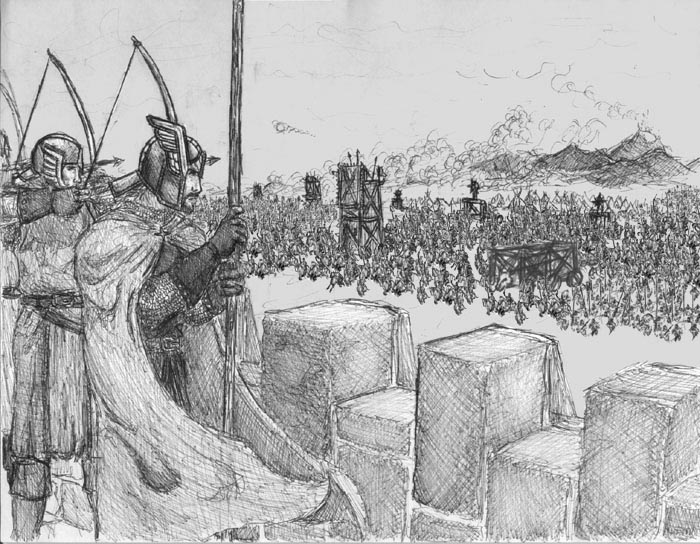
\includegraphics[width=0.75\textwidth]{../images/siege}~
\\[1cm]
\end{center}

\subsubsection{Езда}
\begin{itemize}
\item[-]{нивото на ползване на умения от гърба на кон е ограничено до нивото на умението “езда”}
\item[-]{ръкопашни атаки от и по ездач на галопиращ кон са с двойни щети}
\item[-]{атаки от и по ездач на кон с късо оръжие търпят -5 атака}
\end{itemize}

\subsubsection{Две оръжия}
Едното оръжие се ползва за да нанесе щети на врага, нека наречем него първо.
Второто оръжие може да се ползва за създаване на откриване (което добавя половината боравене в това оръжие към боравенето с основното оръжие) или пък независимо, за пласиране на стопиращи удари (в който случай се ползва независимо, но с наказание -5 на атака).
Ако се атакува само с едното оръжие няма наказания, разбира се.
Щитовете не търпят -5 при пазене.

\subsubsection{Щит}
\begin{itemize}
\item[-]{Щитът е направен да е второ оръжие. Като такъв не търпи -5 когато се ползва за защита.}
\item[-]{пазене от стрели 0/6 (бъклър) през 2/6(кръгъл викингски) през 4/6(дълъг римски) до 6/6 (павис). Това когато активно се криеш от стрелите, разбира се.}
\item[-]{Дървените оръжия и щитове имат здравина 15, а стоманените 30. Това обикновено няма значерние, но силни или бронебойни атаки може да преодолеят успешно блокиране.}
\end{itemize}

\subsection{Таблица щети}
\begin{multicols}{2}
\rowcolors{1}{white}{lightgray}
\begin{tabular}{l | c | c | c}
Сила & *1/2 & *2/3 & *1  \\
1  & d-3  & d-3  & d-2   \\
2  & d-3  & d-2  & d-1   \\
3  & d-2  & d-1  & d-1   \\
4  & d-2  & d-1  & d+1   \\
5  & d-1  & d    & d+2   \\
6  & d-1  & d    & d+3   \\
7  & d    & d+1  & 2d    \\
8  & d+1  & d+2  & 2d+1  \\
9  & d+1  & 2d-1 & 2d+2  \\
10 & d+2  & 2d   & 3d    \\
11 & d+2  & 2d   & 3d+1  \\
12 & 2d-1 & 2d+1 & 3d+2  \\
13 & 2d-1 & 2d+2 & 3d+3  \\
14 & 2d   & 3d-1 & 4d    \\
15 & 2d+1 & 3d   & 4d+1  \\
16 & 2d+1 & 3d+1 & 4d+2  \\
17 & 2d+2 & 3d+1 & 5d    \\
18 & 2d+2 & 3d+2 & 5d+1  \\
19 & 3d-1 & 4d-1 & 5d+2  \\
20 & 3d-1 & 4d   & 5d+3  \\
21 & 3d   & 4d   & 6d    \\
22 & 3d+1 & 4d+1 & 6d+1  \\
23 & 3d+1 & 4d+2 & 6d+2  \\
24 & 3d+2 & 5d-1 & 7d    \\
25 & 3d+2 & 6d   & 7d+1  \\
26 & 4d-1 & 5d   & 7d+2  \\
27 & 4d-1 & 5d+1 & 7d+3  \\
28 & 4d   & 5d+2 & 8d    \\
29 & 4d+1 & 6d-1 & 8d+1  \\
30 & 4d+1 & 6d   & 8d+2
\end{tabular}

\subsection{Масови сражения}
Групи от съюзници могат да бъдат събирани в "строй".
Не е нужно групата да е хомогенна, но трябва да имат обща цел.

\subsubsection{Характеристики на строй}
\begin{itemize}
% Структурни
\item{Лице - брой бойци с достъп до врага.}
\item{Гъстота - от 1:1 (стена от щитове) до 1:5 (цвайхендери)}
\item{Връхлитане - х1.5 за пешаци, х3 за конница}
\item{Придвижване - равно на придвижването на най-бавният.}

% Състояние
\item{Брой живи - бойци в добро здраве.}
\item{Брой ранени - небоеспособни, в ръцете на леакрите след битка.}
\item{Морал - равен на Дисциплина(Инт), спадне ли до 0, строят се превръща в "тълпа".}

% Компетентност и екипировка
\item{Ръкопашен бой - Сила + най-високото боравене с налично ръкопашно оръжие.}
\item{Стрелба - Сила + най-високото боравене с налично далечно оръжие}
\item{Броня - Сила + (1/10)сума(пазене * здравина), без щитове}
\end{itemize}
\end{multicols}
\subsubsection{Правила}
Ръкопашен бой + д6* с/у броня. Ако нападащият строй спечели, лицето на строят му се нанася 1/2 като убити и 1/2 като ранени върху противника. Разликата в хвърлянето се нанася върху моралът на противника / противника губи 1 точка морал (\textit{кое е по-добро?}).

Директна стрелба (под 1 инкремент на оръжието) следва правилата за ръкопашен бой. Стрелба до максималното разстояние на хвърляне на оръжието е на половина щета.

Лице и Дълбочина. Един строй може да бъде нападнат едновременно от най-много толкова строеве, сумата от чиито лица е колкото два пъти лицето на  нападнатите.

Ако броят живи спадне под числото лице, строят се разпада (превръща се в тълпа).

Ранените бойци са боеспособни, но намалят придвижването на стоя на половина. Лекуването им отнема половин месец.

Морал. При виждане на разбиване на приятелски сторй, или ако бягащ разбит строй премине през позициите на друг строй, морал се намаля с 1.

При морал 0, строят се разбива и се превръща в тълпа.

Войници не в строй (а в тълпа) търпят наказание на всичко от -5.

При виждане на поне двойно числено превъзхождащ противник, всеки строй губи 1 морал.

При виждане на подготвящ се да връхлети двойно по-многоброен или много по-добре екипиран строй, строят губи 1 морал.

Моралът се възстановява извън битка с 1 точка на минута.
